\documentclass[]{article}%falls andere Sprache als "ngerman", bitte hier als Option einfügen (bspw. english oder british)
\usepackage{aale}
% Die folgenden beiden Pakete werden für Bilder und schönere Tabellenlinien benötigt.
% Falls aale.cls sie bereits laedt, ist das erneute Laden unschädlich.
\usepackage{graphicx}
\usepackage{booktabs}
\usepackage{url} % fuer \url{} in den Literaturangaben

\title{Factory Control Unit}
\runningtitle{Factory Control Unit}
\subtitle{Modellgetriebene Steuerung für die Lernfabrik Factory-in-a-Box}

\author{1}{Klaus M. Liebler}


\affil{1}{Hochschule Osnabrück, Fakultät für Ingenieurwissenschaften und Informatik, Osnabrück, Deutschland}

\confno{23}
\confdate{17.--19. März\ }
\confyear{2027}
\confplace{Fulda}

\logofile{logo}%Das richtige Logo aus Verzeichnis Logos_Lizenz unter Bezeichung "logo.eps" in das Hauptverzeichnis kopieren.

\begin{document}
\setcounter{page}{1}
\maketitle


\abstract{Lernfabriken machen Automatisierungstechnik greifbar und werden in berufsbildenden Schulen und Hochschulen der angewandten Wissenschaften in praxisorientierten Lehrformaten eingesetzt. Factory-in-a-Box (FiaB) ist ein weiteres Konzept in diesem Umfeld, das einen neuen Kompromiss zwischen Vielfalt, Kosten und Einsatzbereich anstrebt. Der Beitrag stellt zunächst kurz die wesentlichen Änderungen am Prozesskonzept gegenüber \cite{liebler2025} vor. Im Fokus steht anschließend die Factory Control Unit (FCU), die eingebettete elektronische Zentralsteuerung von FiaB.}

\keywords{Factory-in-a-Box, Factory Control Unit, Lernfabrik, Modellgetriebene Entwicklung, Eingebettete Systeme}


\section{Stand der Technik}

Für die berufliche Bildung und die Hochschullehre existiert eine Reihe kommerzieller Lehraufbauten, die jedoch selten sämtliche in Kapitel~2 formulierten Anforderungen gleichzeitig erfüllen. Die \emph{fischertechnik Training Factory} \cite{fischertechnik} bildet mit den aus dem Baukastensystem bekannten Komponenten verschiedene Abläufe eines Industrieunternehmens spielerisch nach, wobei industrietypische Technik nur in geringem Umfang zum Einsatz kommt. Festo Didactic bietet demgegenüber ein breites Spektrum modularer, industrienaher Lernfabriken an, deren Module üblicherweise kundenspezifisch konfiguriert werden; vergleichbare, jedoch stärker auf einzelne Regelkreise als auf einen Gesamtprozess ausgerichtete Systeme vertreibt beispielsweise auch GUNT. Die Anschaffungskosten dieser industrienahen Systeme liegen typischerweise zwischen 20.000\,€ und über 100.000\,€, wodurch sich eine Mehrfachbeschaffung für Kleingruppen- oder Einzelarbeitsplätze kaum wirtschaftlich realisieren lässt.

Einen deutlich kostengünstigeren, primär auf den schulischen Unterricht zugeschnittenen Weg verfolgt das an den Berufsbildenden Schulen Osnabrück entwickelte \emph{Smart Factory Model} \cite{strating2023}: Eine reale speicherprogrammierbare Steuerung steuert einen kompakten Portalroboter, während ein in den Arbeitsbereich integrierter Bildschirm den Shopfloor virtuell darstellt und so einen schnellen Wechsel zwischen unterschiedlichen Prozessen ermöglicht; die Kosten für einen vollständigen Aufbau belaufen sich auf etwa 6.000\,€.

Das in diesem Beitrag betrachtete Konzept \emph{Factory-in-a-Box} (FiaB) wurde von Liebler \cite{liebler2025} als kompakte, mobile und kostengünstige Modellfabrik vorgestellt, die einen vereinfachten industriellen Produktionsprozess anschaulich macht: einen Kreislaufprozess farbiger Holzklötze, aus denen kundenindividuelle Türme gefertigt werden. Der gesamte Aufbau wird als Open-Source-Projekt bereitgestellt, sodass Nachbau, Anpassung und Weiterentwicklung durch Dritte ausdrücklich vorgesehen sind. Gegenüber den zuvor genannten Systemen ordnet sich FiaB damit sowohl hinsichtlich der Anschaffungskosten als auch hinsichtlich Bauraum und Beweglichkeit am unteren Ende des Spektrums ein (vgl. Kapitel~\ref{sec:evaluation}).

\section{Anforderungen und Architektur}

An die Modellfabrik \emph{Factory-in-a-Box} wurden die folgenden wesentlichen Anforderungen gestellt:

\begin{itemize}
\item Darstellung eines vereinfachten industriellen Produktionsprozesses
\item Einsetzbarkeit in verschiedenen Vorlesungsmodulen der Automatisierungstechnik
\item vielfältige Sensorik und Aktorik
\item vielfältige Kommunikationsschnittstellen
\item niedrige Investitions- und Betriebskosten
\item mechanisch und elektrisch robust (Außenrahmen, verpolungssicherer USB-C-Anschluss)
\item kompakt und mobil
\end{itemize}
% Hinweis: Der ursprüngliche Entwurf enthielt einen leeren letzten Punkt ("\item" ohne Text).
% Ich habe ihn entfernt -- falls dort noch eine Anforderung fehlt, bitte ergänzen.

Die Anforderungen wurden hinsichtlich Mechanik, Elektronik und Software wie folgt umgesetzt.

\subsection{Mechanischer Aufbau}
Die derzeitige Umsetzung basiert im Wesentlichen auf dem in \cite{liebler2025} vorgestellten Konzept: einem Kreislaufprozess farbiger Holzblöcke. Produkt der Fabrik sind kundenindividuell gefertigte Türme aus diesen Holzklötzen. Eine wesentliche Erweiterung gegenüber dem ursprünglichen Konzept ist ein Pneumatiksystem, das die Holzklötze auf das Förderband auflegt: Es ersetzt den zuvor eingesetzten Servoantrieb durch ein weiteres, industrietypisches System und ermöglicht zugleich die Druckregelung als Thema der Regelungstechnik. Außerdem wurde der Greifer am Roboter durch einen Vakuum-Saugnapf ersetzt, was ein weiteres interessantes System einführt und die Betriebssicherheit erhöht. Darüber hinaus sollen RGB-LED-Streifen in den senkrechten Stützen als Fehlermeldeleuchte dienen und alternativ Prozessgrößen unmittelbar visualisieren.

\subsection{Elektronisches Konzept}
Die wachsende Vielfalt der integrierten Komponenten und die Anforderung nach innovativen Kommunikationsschnittstellen machten es erforderlich, von Lab@Home als zentraler Steuerungskomponente Abstand zu nehmen. Eine eigene Steuerplatine auf Basis eines STM32H5-Mikrocontrollers bindet stattdessen alle Sensoren und Aktoren an und stellt diverse Kommunikationsprotokolle bereit -- sowohl für smarte Sensoren und Aktoren als auch in Richtung der übergeordneten Steuerungsebene.

\subsection{Softwarearchitektur}
Die C++-Firmware (C++20) basiert auf Eclipse ThreadX \cite{threadx} als Echtzeitbetriebssystem und nutzt zusätzlich NetX Duo (für TCP/IP, TLS, DHCP, mDNS) sowie USBX (für CDC-ACM zur Realisierung von Modbus RTU sowie für CDC-NCM). Die Firmware orchestriert alle Sensoren und Aktoren, stellt verschiedene Kommunikationswege zur Außenwelt bereit und pflegt ein zentrales Informationsmodell.

\subsection{Software-Build-Prozess}
Zur Erstellung des Binärabbildes der Software ist es -- ähnlich wie bei Lab@Home \cite{liebler2023} -- erforderlich, dass mehrere Schritte koordiniert nacheinander ablaufen. Bei Lab@Home wurde hierfür ein Gulp-Skript eingesetzt. Für die FCU wurde stattdessen ein eigenes Build-Tool auf Basis von .NET entwickelt.
% KI-Ergaenzung (wie im Auftrag markiert): Ich habe unten einen Satz zur KI-Unterstuetzung
% bei der Entwicklung des Build-Tools ergaenzt. Da ich die genauen Details (welches Werkzeug,
% welche Teile) nicht kenne, ist die Formulierung bewusst allgemein gehalten -- bitte pruefen
% und ggf. praezisieren oder mit einer konkreten Angabe (z. B. verwendetes Modell/Tool) versehen.
Die Entwicklung erfolgte KI-unterstützt: Ein KI-Assistent half unter anderem beim Architekturentwurf, bei der Codegenerierung sowie bei der Fehlersuche und verkürzte damit die Entwicklungszeit spürbar. Die Gründe für diese Werkzeugwahl werden im Folgenden erläutert.

\section{Implementierung}

\subsection{Details zum Informationsmodell}
Das Prozessabbild ist einmalig als annotierte \texttt{C\#}-Klassen beschrieben (Abb.~\ref{fig:informationsmodell}): 16 Klassen bilden Regionen, 75 Felder Register. Attribute legen Zugriffsrecht, Einheit, Registeradresse, Pin, Wertebereich und Darstellungsart fest; auch Bitfelder und 32-Bit-Werte aus Registerpaaren lassen sich beschreiben. Ein neu entwickelter Generator in \texttt{C\#} (UniversalRegisterAccess), vom .NET-Build-Orchestrator aufgerufen, erzeugt daraus drei Artefakte: (1) einen \texttt{C++}-Header für Modbus mit Adresskonstanten, Regionsgrenzen, Bitmasken und typisierten Accessoren; (2) eine constexpr-Knotentabelle für OPC UA (ein Objekt je Region, eine Variable je Register mit Datentyp, Zugriffsrechten und Callbacks), die ohne Laufzeitaufbau im Flash liegt; sowie (3) eine TypeScript-Registerkarte, aus der das Web-UI seine generischen Register-Panels (Tabellen, Schalter, Schieberegler mit Grenzen) rendert. Schemaänderungen wirken so gleichzeitig auf Firmware und Oberfläche; Inkonsistenzen zwischen den Sichten werden bereits zur Übersetzungszeit vermieden.

\begin{figure}[htbp]
\centering
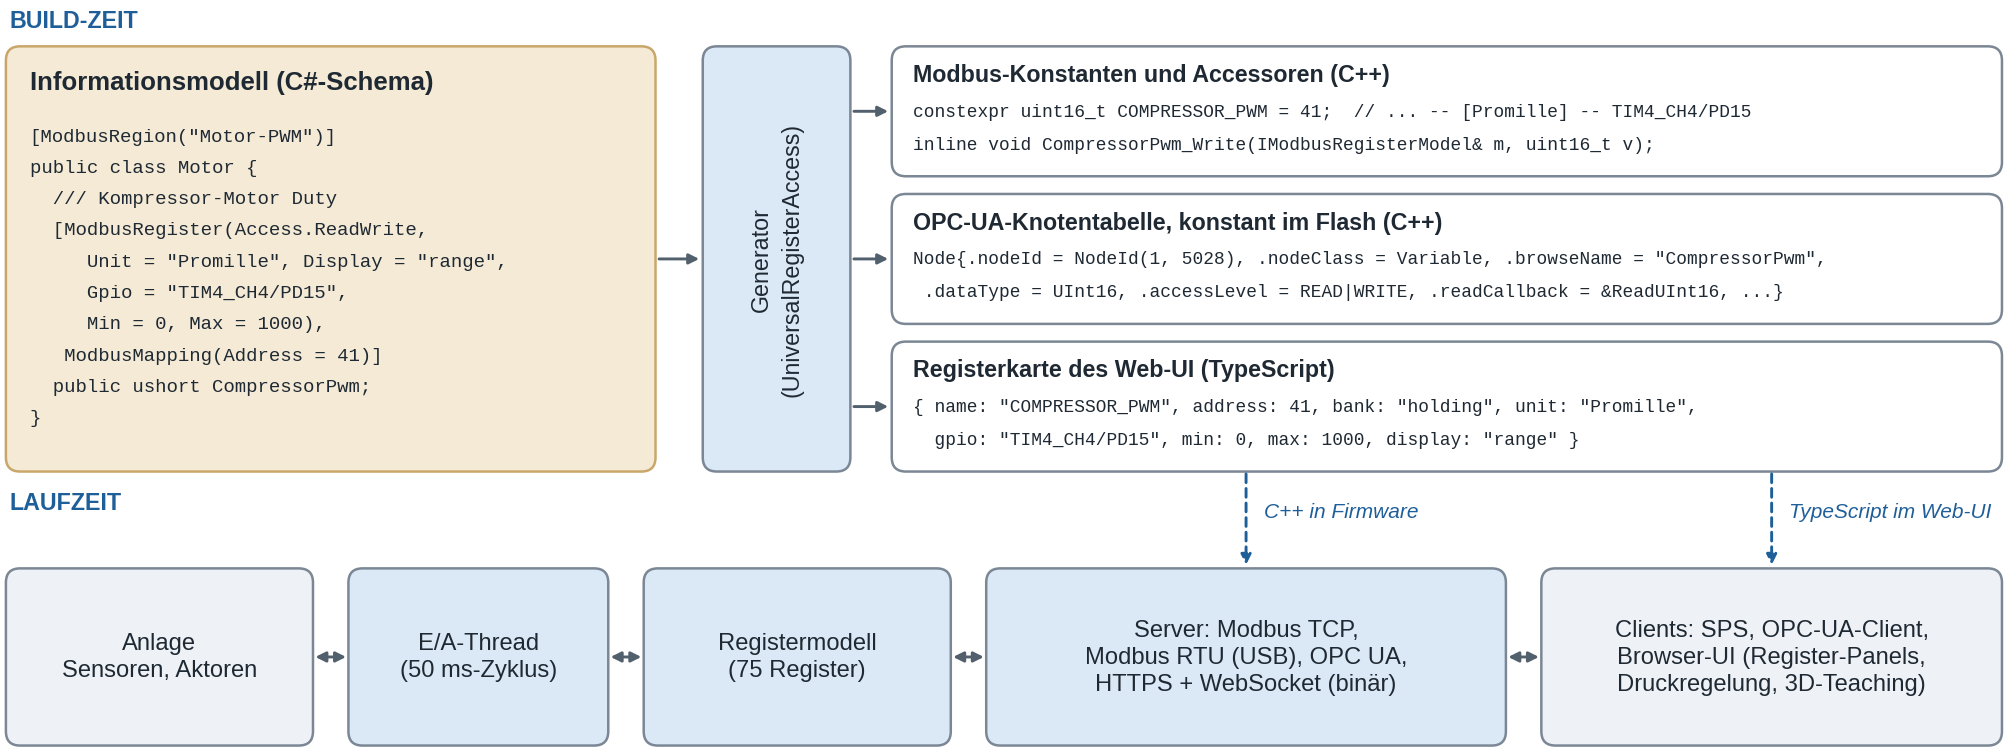
\includegraphics[width=\linewidth]{fig1_informationsmodell.png}
\caption{Informationsmodell und Laufzeitarchitektur der FCU: Ein C\#-Schema wird durch einen Generator in Modbus-, OPC-UA- und Web-UI-Code übersetzt; zur Laufzeit teilen alle Zugriffswege ein gemeinsames Registermodell.}
\label{fig:informationsmodell}
\end{figure}

Ein zweites Schema (BestBinaryBuffers) beschreibt rund 30 Nachrichten des WebSocket-Protokolls samt Union-Typen für Missionsschritte und Längengrenzen und erzeugt Kodierer, Dekodierer und maximale Puffergrößen für C++ und TypeScript.
% Hinweis: Der urspruengliche Verweis "(Tab. 1)" am Satzende habe ich entfernt, da dieses
% Dokument keine Tabelle der generierten Dateien enthaelt (nur die Tabelle zum Lehreinsatz,
% s. Abschnitt "Einsatz in der Lehre"). Falls gewuenscht, baue ich eine solche Tabelle analog
% zur Kurzfassung wieder ein.
Der Orchestrator leitet je Board Hostname und MAC-Adresse aus der Chip-UID ab, erzeugt das TLS-Zertifikat, baut Web-UI (Vite) und Firmware (CMake) und flasht; das Preset Debug-Nucleo erlaubt die Arbeit auf einem Nucleo-H563ZI-Testboard.


\subsection{Details zur Hardware}
Die vierlagige Platine vereint einen STM32H563 (Cortex-M33, 640 KiB RAM) mit Ethernet, zwei USB-C-Anschlüssen (Device, Power-Delivery-Sink) und FDCAN. Für die Anlage sind zwei Schrittmotortreiber (TMC2209, sensorloses Homing), ein Wägezellenwandler, drei Abstands- und ein Farbsensor (I²C), ein Leistungsmonitor (INA226), Lichtschranken, Ventil- und PWM-Treiber, ein Drucksensoreingang, eine Statusbeleuchtung sowie ein Bus-Servo-Anschluss für den Roboterarm vorgesehen. Ein EtherCAT-Slave-Controller (LAN9253) ermöglicht bei Bedarf auch die Implementierung dieses echtzeitfähigen Protokolls.
% TODO: Der Satz zu den USB-C-Anschluessen brach im Entwurf mitten im Wort ab ("Die USB").
% Ich habe ihn entfernt statt etwas zu erraten -- bitte den Gedanken ergaenzen.

Die elektronische Baugruppe ist auf einer Leiterplatte aufgebaut, die sich direkt mit den horizontalen oberen Streben verschrauben lässt. Die Platinenunterseite trägt alle SMD-Bauteile, die von einem chinesischen Platinenfertiger unmittelbar bestückt werden; die Oberseite enthält von Hand zu bestückende THT-Buchsen sowie umfangreiche Beschriftungen. Die Stromversorgung kann wahlweise über ein 24-V-Netzteil (Klinkenstecker) oder über ein USB-PD-Netzteil (20\,V, 100\,W) erfolgen.

\subsection{Details zur Firmware}
Kernaufgabe der Firmware ist die Initialisierung der Hardware und die Herstellung der Betriebsbereitschaft. Im laufenden Betrieb bedienen mehrere unabhängige Tasks alle Kommunikationsprozesse und steuern die Hardware an. Dabei laufen folgende Kommunikationsprozesse:
\begin{itemize}
\item Konsolenausgabe des Logs
\item Modbus-TCP-Server, erreichbar über Ethernet und über einen virtuellen Netzwerkadapter an der USB-C-Schnittstelle (USB CDC-NCM)
\item OPC-UA-Server (Basic256Sha256 im Modus Sign), ebenfalls erreichbar über Ethernet und den virtuellen Netzwerkadapter
\item Modbus-RTU-Server, erreichbar über Ethernet und über eine virtuelle serielle Schnittstelle an der USB-C-Schnittstelle (USB CDC)
\item SNTP-Client zum Bezug der Echtzeit
\item HTTPS-Server zur Bereitstellung des Browser-Clients und einer RESTful API
\item HTTPS-WebSocket-Server für die laufende Kommunikation zwischen Browser und Baugruppe
\item synchronisierte Ansteuerung der Antriebe des 6-DOF-Roboters über ein Bus-Servo-Protokoll
\item USB-PD-Sink zur Anforderung von 20\,V oder 28\,V (PD 3.1) von einem entsprechend kompatiblen USB-PD-Netzteil
\end{itemize}

Der OPC-UA-Server ist als ressourceneffiziente Eigenentwicklung (rund 3900 Zeilen C++) entstanden. Hinsichtlich der Sicherheit unterstützt er derzeit Basic256Sha256 im Modus Sign. Eine Besonderheit: Der Namespace~0 enthält überwiegend konstante Werte und liegt daher als konstante Tabelle im Flash; nur die wenigen volatilen Werte verweisen auf Speicherorte im RAM. Zur Laufzeit wird dafür kaum RAM benötigt. OPC UA und HTTPS-Server teilen sich ein gemeinsames X.509-Zertifikat.

\section{Details zum Webfrontend}
Das Web-UI ist eine Single-Page-Anwendung aus Lit-Web-Components (TypeScript, Vite), die als whitespace-minimierte, obfuskierte und Brotli-komprimierte Datei (84\,kB statt 460\,kB) per HTTPS aus dem Flash der FCU ausgeliefert wird. Alle Anwendungsdaten werden anschließend ausschließlich über einen binären WebSocket ausgetauscht. Folgende Seiten sind erreichbar:
\begin{itemize}
\item Registermodell: lesender und schreibender Zugriff auf alle im Informationsmodell definierten Register über typgerecht gerenderte Eingabefelder und Schalter
\item Power Monitoring mit aktueller Versorgungsspannung, Strom, Momentanleistung und Leistungshistorie
\item Task-Manager mit ThreadX-Live-Statistik
\item Roboter-Missionsplanung
\item Druckregelkreis: Identifikation und Charakterisierung einer Druckregelstrecke sowie Parametrierung eines PID-Reglers
\end{itemize}

Die Seiten \textbf{Druckregelkreis} und \textbf{Roboter-Missionsplanung} haben besondere Bedeutung in der Lehre des Autors und werden deshalb im Folgenden ausführlicher beschrieben.

\subsection{Druckregelstrecke}
Die Druckregelstrecke besteht aus Kompressor, Kessel, einem realen Verbraucher (Doppelkolbenzylinder), drei simulierten Verbrauchern (Ventile mit Drossel) und einem Drucksensor. Die Weboberfläche bietet vollständig integrierte Möglichkeiten zur Kennlinienerstellung und zur dynamischen Analyse mittels des klassischen Sprungantwortversuchs (Auswertung nach dem Wendetangentenverfahren).

Im Vergleich zu den zuvor im Labor verwendeten Regelstrecken \emph{Heizwiderstand} und \emph{Schwebekörper} zeichnet sich die Druckregelstrecke durch eine gute Linearität in einem weiten Arbeitsbereich und ein angenehmes Zeitverhalten aus (Zeitkonstante etwa 20\,s). Die Studierenden erhalten auf Wunsch programmintegrierte Unterstützung bei der Ermittlung von Arbeitspunkt, Proportionalitätsfaktor, Totzeit und Zeitkonstante. Die Werte lassen sich unmittelbar in eine Berechnungshilfe nach der T-Summen-Regel nach Kuhn oder nach Chien--Hrones--Reswick \cite{chien1952} übertragen, die ihrerseits die Ergebnisse in die Parameterfelder eines P-, PI- oder PIDT1-Reglers überträgt. Der Regelalgorithmus läuft dabei im Browser, der über Lesen und Beschreiben des Registermodells mit Drucksensor sowie realem und simulierten Verbrauchern kommuniziert.

\subsection{Roboter-Missionsplanung}
Factory-in-a-Box integriert den 6-DOF-Roboter RoArm M3 zur Verbringung von Holzklötzen aus einem Durchlaufregal zu einer Montageplattform für Klötzchentürme. Inspiriert von MoveIt2 wurde eine für den verwendeten Roboter maßgeschneiderte, vollständig webbasierte Lösung entwickelt, bei der 3D-Geometriedaten und Bewegungsachsen fest einkompiliert sind. Diese Lösung stellt den Roboter in 3D innerhalb von FiaB dar und ermöglicht über einen Gizmo eine einfache Positionierung und Ausrichtung. Jede Pose lässt sich als Schritt in einer Robotermission speichern; daneben können auch Schritte zum Aktivieren oder Deaktivieren des Vakuum-Saugnapfs sowie Wartezeiten hinzugefügt werden. Eine Mission wird dann unter einem Namen und einem individuellen Missionsindex in einem kleinen Dateisystem auf der FCU persistiert und lässt sich über eben diesen Index aus dem Registermodell heraus aufrufen. Als technische Basis für die 3D-Ansicht läuft ein PBR-Shader, der über das schlanke OGL auf die WebGL-Implementierung des Browsers zugreift. Eine geschlossene, nicht iterative inverse Kinematik ist sowohl im Browser als auch zur Ausführung der Missionen in der Firmware implementiert.

\begin{figure}[htbp]
\centering
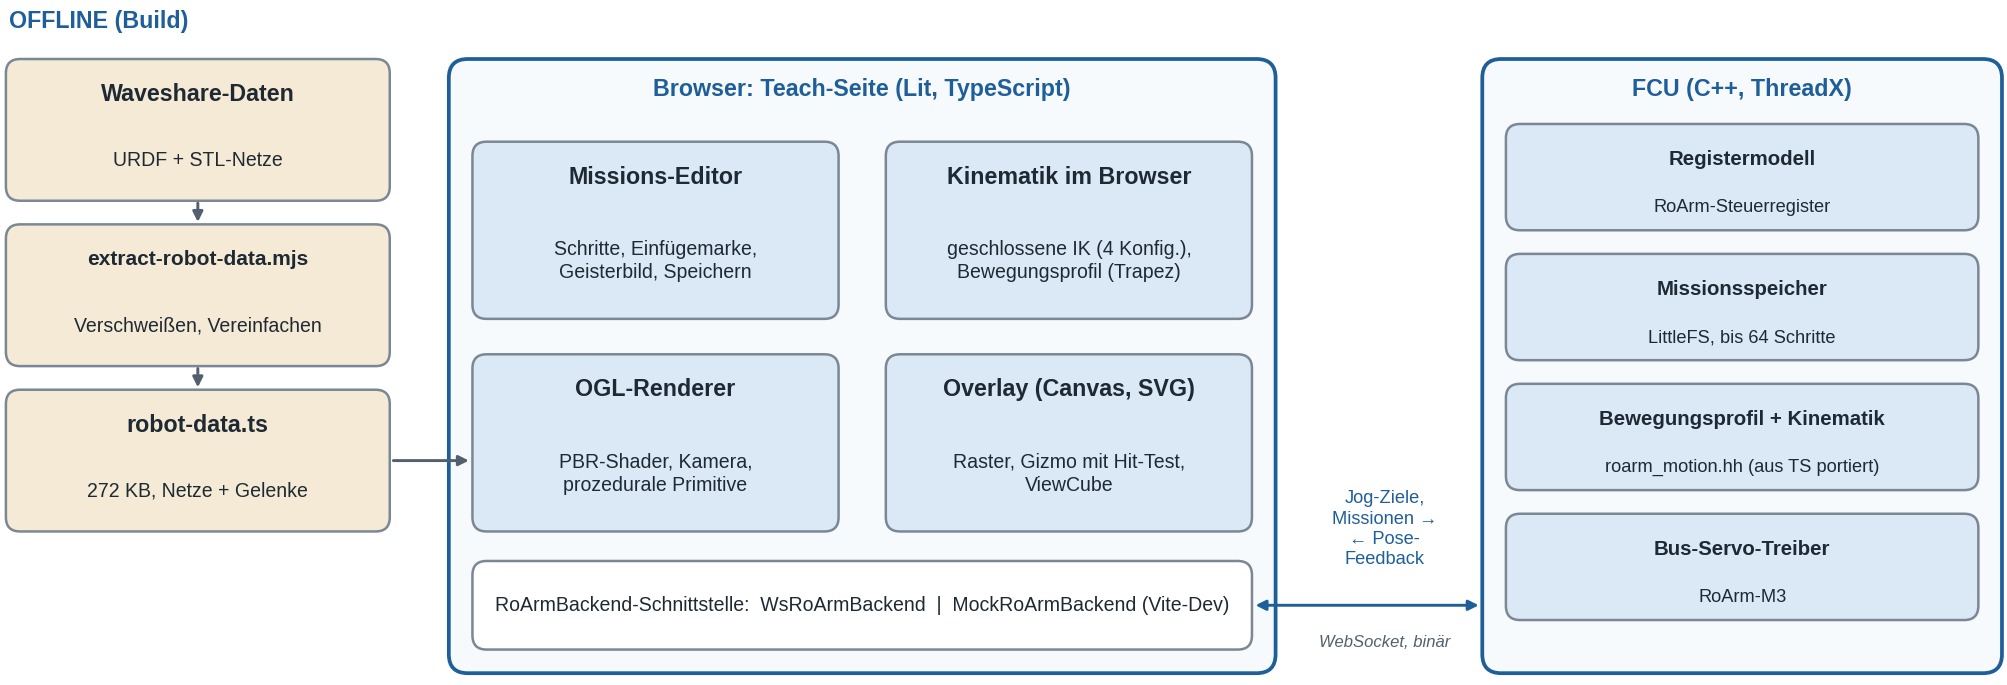
\includegraphics[width=\linewidth]{fig2_teach_architektur.png}
\caption{Teach-Seite: Roboterdaten aus der Offline-Werkzeugkette, Browser-Komponenten und Kopplung zur FCU über eine Backend-Schnittstelle.}
\label{fig:teach-architektur}
\end{figure}

\begin{figure}[htbp]
\centering
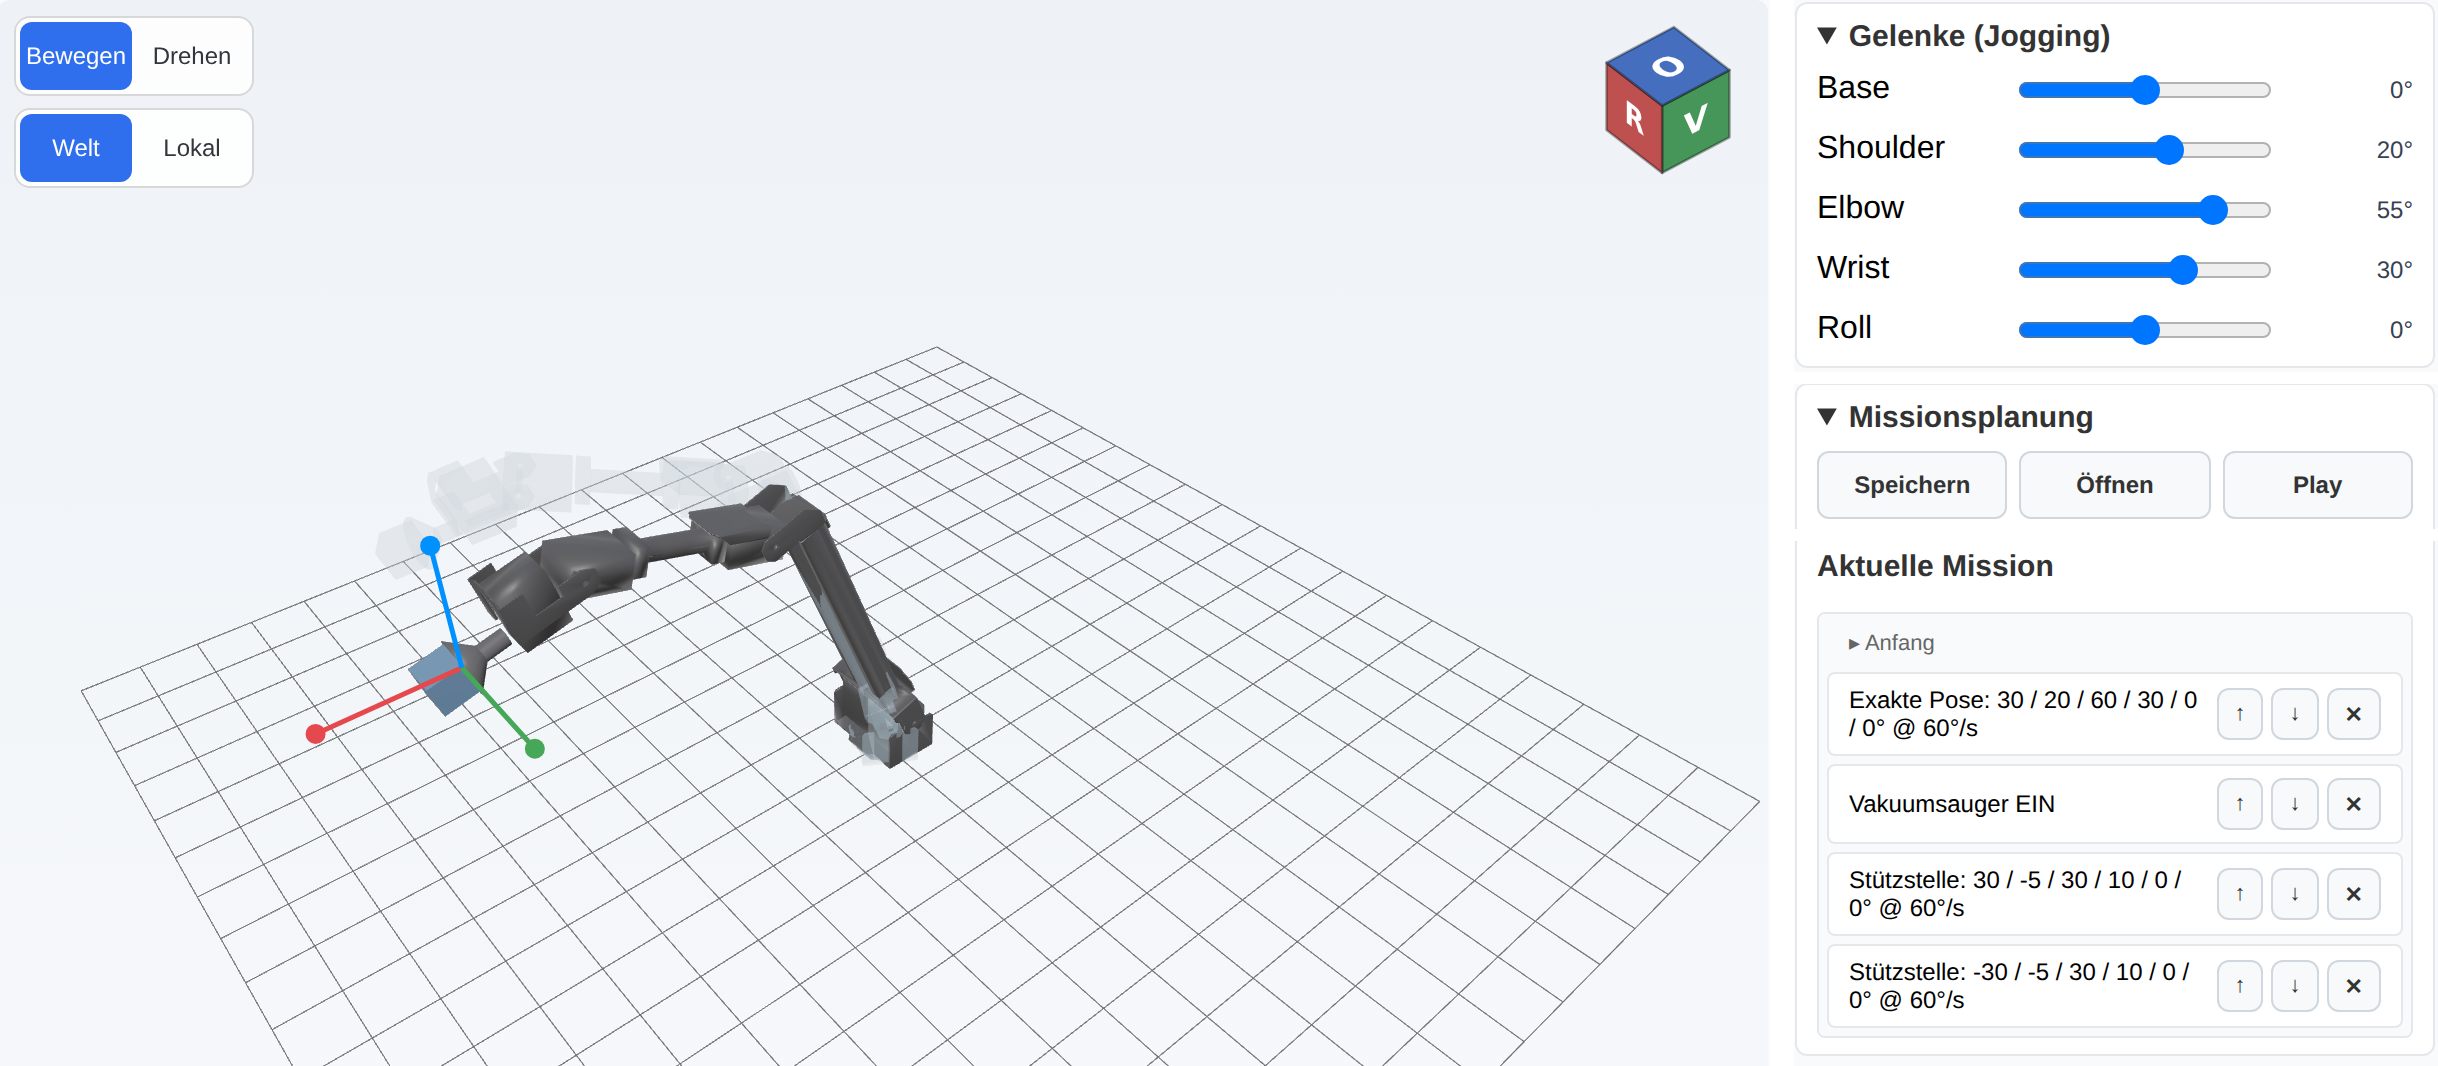
\includegraphics[width=0.75\linewidth]{fig3_teach_screenshots.png}
\caption{Teach-Seite (Ausschnitte): 3D-Modell mit Gizmo, ViewCube und Geisterbild; Gelenkschieber und Missionsliste (Entwicklungsserver, Mock-Backend).}
\label{fig:teach-screenshots}
\end{figure}

\section{Details zum Build-Prozess}
Zur Orchestrierung des Build-Prozesses wurde ein neues Build-Tool in .NET entwickelt. Ausschlaggebend für diese Entscheidung war, dass zur Beschreibung des Informationsmodells und der Nachrichtenstrukturen zwischen Browser-Frontend und HTTPS-WebSocket-Server annotierte \texttt{C\#}-Klassen zum Einsatz kommen sollten. Da für das Parsen und die Umwandlung dieser Klassen ohnehin eine .NET-Umgebung erforderlich war, erschien es aus Effizienzgründen sinnvoll, dieses Framework auch für die gesamte Build-Orchestrierung zu verwenden. Ein ausführliches Log und eine farbige Konsolenausgabe während des Builds schaffen dabei Transparenz und Nachverfolgbarkeit:
\begin{enumerate}
\item Auslesen der eindeutigen Chip-ID über das Debugging-Interface oder den seriellen Bootloader
\item Erstellung eines gerätespezifischen Zertifikats für OPC UA und HTTPS
\item Codegenerierung für einkompilierbare Informationen über die Hardware-ID der Baugruppe und daraus abgeleitete Größen
\item Codegenerierung für den einkompilierten Verweis auf den verwendeten Repository-Stand
\item Codegenerierung für das Informationsmodell auf Basis der annotierten \texttt{C\#}-Klassen; der generierte Code wird vom OPC-UA-Server, von beiden Modbus-Servern und vom Webclient zum Aufbau der Strukturen verwendet
\item Codegenerierung der Encoder und Parser für die Kommunikation zwischen HTTPS-WebSocket-Server und Browser-Client, ebenfalls auf Basis annotierter \texttt{C\#}-Klassen
\item Bau des Browser-Clients (Vite-Applikation, anschließend Single-File-Inlining, Whitespace-Elimination und Brotli-Kompression)
\item Bau der Firmware, wobei Zertifikate und Browser-Client in das Binary eingelinkt werden
\end{enumerate}


\section{Einsatz in der Lehre}

Die FCU soll in vier Lehrveranstaltungen eingesetzt werden (Tab.~\ref{tab:lehrveranstaltungen}). Alle arbeiten an derselben, greifbaren Anlage, setzen aber an unterschiedlichen Schnittstellen an.

\begin{table}[htbp]
\centering
\small
\caption{Geplanter Einsatz der FCU in vier Lehrveranstaltungen.}
\label{tab:lehrveranstaltungen}
\begin{tabular}{p{0.20\linewidth}p{0.33\linewidth}p{0.37\linewidth}}
\toprule
\textbf{Veranstaltung} & \textbf{Lerninhalte} & \textbf{Nutzung der FCU und Aufgaben} \\
\midrule
Connected Systems (Master) & Kommunikationsgrundlagen, Signierung und Verschlüsselung in OPC UA, Echtzeitprotokoll EtherCAT & Modbus und OPC UA (Basic256Sha256, Sign, Gerätezertifikat) auf einem Prozessabbild; EtherCAT-Slave (LAN9253); Mitschnitte und Zertifikate untersuchen \\[2pt]
Regelungstechnik & Streckenidentifikation, Reglerentwurf, Anti-Windup & Druckregelstrecke: Kennlinie, Sprungantwort, Reglerbetrieb (P/PI/PID); Regler einstellen und vergleichen \\[2pt]
Automatisierungs\-technik & IEC 61131-3, Ablaufsprache (AS), Funktionsbausteinsprache (FBS) & Fabrik als reale Anlage; Soft-SPS (z.\,B. CODESYS) über OPC UA oder Modbus; Sortier- und Transportablauf, Inbetriebnahme \\[2pt]
Embedded Systems & Hardwarenaher Entwurf, Echtzeitbetriebssystem, Treiber & Modulare Platine, Testboard Nucleo-H563ZI, reproduzierbarer Build; Baugruppe oder Submodul weiterentwickeln \\
\bottomrule
\end{tabular}
\end{table}

\subsection{Master-Vorlesung „Connected Systems“}
Die FCU dient als Anschauungsobjekt für Kommunikation, Absicherung und Echtzeitfähigkeit. Zunächst werden Kommunikationskonzepte (Master/Slave, Client/Server, Registerabbild gegenüber Informationsmodell) an Modbus und OPC UA auf demselben Prozessabbild verglichen. Für OPC UA wird das Sicherheitskonzept praktisch nachvollzogen: Der Server nutzt Basic256Sha256 im Modus Sign mit gerätespezifischem Zertifikat; Studierende untersuchen Zertifikate und Vertrauenskette, stellen im Netzwerkmitschnitt fest, dass signierte Nachrichten manipulationsgeschützt, aber lesbar sind, und diskutieren den Schritt zu Sign and Encrypt \cite{iec62541}. Als Echtzeitprotokoll dient EtherCAT \cite{ethercat}: Der Slave-Controller der Platine wird in einen Verbund aufgenommen, Zykluszeit und Determinismus werden mit Modbus und OPC UA verglichen.
\subsection{Regelungstechnik: Druckregelstrecke}
Die Druckregelstrecke hat eine nichtlineare, über die Ventilkombination veränderliche Kennlinie und deckt den Weg von der Identifikation bis zum Regler ab: Studierende nehmen Kennlinien auf, bestimmen aus Sprungantworten Totzeit und Zeitkonstante, entwerfen P-, PI- und PID-Regler nach Einstellregeln und beobachten im realen Regelkreis Stellgrößenbegrenzung und Anti-Windup. Da der Regelkreis nur über Register geschlossen wird, kann der Regler auch in einem Skript oder einer SPS laufen.
\subsection{Automatisierungstechnik: Steuerungsentwurf nach IEC 61131-3}
Die Fabrik ist der Prozess, für den Studierende die Steuerlogik nach IEC 61131-3 \cite{iec61131} entwickeln, wahlweise in Ablaufsprache (AS) oder Funktionsbausteinsprache (FBS), etwa in CODESYS als Soft-SPS. Die Kommunikation mit der Fabrik erfolgt über OPC UA oder Modbus, sodass beide Wege verglichen werden können. Typische Aufgaben sind ein Sortier- und Transportablauf mit Förderband, Lichtschranken, Ventilen und Sensoren sowie der Aufruf von Roboter-Missionen als Teilablauf; die Register-Panels dienen der Inbetriebnahme.
\subsection{Embedded Systems: Weiterentwicklung von Baugruppen}
Die Platine gliedert sich in funktionale Baugruppen (Antriebe, I²C-Sensorik, Leistungserfassung, Ventil- und PWM-Ausgänge, Kommunikation); Studierende können einzelne Baugruppen oder Submodule weiterentwickeln, etwa einen Sensorzweig, eine Treiberstufe oder eine Erweiterungsplatine samt Firmware-Treiber. Reproduzierbarer Build und Nucleo-H563ZI-Testboard erlauben Arbeit ohne eigene Platine; neue Register stehen nach Ergänzung im Schema in Modbus, OPC UA und Web-UI bereit.


\section{Evaluation}
\label{sec:evaluation}
Die grundsätzliche Funktion der Mechanik und der Elektronik der FCU wurde im Rahmen studentischer Abschlussarbeiten geprüft. Firmware und Build-Prozess sind implementiert und anhand von Unit-Tests geprüft. Offen sind konkrete Aufgabenformulierungen in allen Modulen sowie das Einholen von Feedback der Studierenden. Die Materialkosten pro Einheit belaufen sich auf etwa 750--850\,€, wobei ein wesentlicher Teil auf den Roboter entfällt.

Zum Konferenzthema Energiemonitoring liefert der INA226 Spannung, Strom und Leistung der Anlage über alle Schnittstellen; in der Lehre lassen sich Ablaufvarianten energetisch vergleichen. Für Praxis und Forschung zeigt der Ansatz, wie ein Informationsmodell konsistente Feldbus-, OPC-UA- und Web-Sichten aus einer Quelle erzeugt und dabei auf einem preiswerten Mikrocontroller Platz findet.
% Hinweis: Eine leere Aufzaehlung (\begin{itemize}\item\end{itemize}) stand hier im Entwurf;
% ich habe sie entfernt. Falls dort noch Stichpunkte folgen sollten, bitte ergaenzen.

\section{Geplante Weiterentwicklung bis zur AALE}
Angesichts des Fokus der AALE 2027 soll dieser Bereich noch dahingehend erweitert werden, dass die Leistung in den Kontext der aktivierten Verbraucher gesetzt wird und so eine verursachergerechte Zuordnung und damit eine effiziente Reduktion des Energieverbrauchs möglich wird.
% TODO: Der Absatz brach im Entwurf hier mitten im Satz ab ("Die An..."). Bitte vervollstaendigen.

Die Fortentwicklung von EtherCAT wird zunächst niedriger priorisiert, da es gegenwärtig keinen konkreten Einsatzfall dafür gibt.

\section{Literatur}

\bibliographystyle{plain}
\bibliography{references}

\end{document}
